\documentclass[aspectratio=169]{beamer}
\usepackage[utf8]{inputenc}
\usepackage{hyperref}
\usepackage{amsmath,amsfonts,amsthm,bm}
\usepackage{color}
\usepackage{graphicx} % Allows including images
\usepackage{subcaption}
\usepackage{booktabs} % Allows the use of \toprule, \midrule and \bottomrule in tables
\usepackage{tikz}
%\usepackage{pgfplots}
\usepackage{listings}
\usepackage{courier}
\usepackage[version=4]{mhchem}
\usepackage{array}

\lstset{ %
    basicstyle=\scriptsize\ttfamily, % fonts that are used for the code
    breakatwhitespace=false,         % sets if automatic breaks should only happen at whitespace
%breaklines=true,                 % sets automatic line breaking
%captionpos=b,                    % sets the caption-position to bottom
    commentstyle=\color{gray}\textit,    % comment style
    keepspaces=true,                 % keeps spaces in text, useful for keeping indentation of code (possibly needs columns=flexible)
    keywordstyle=\color{blue},       % keyword style
    language=Python,                 % the language of the code
%otherkeywords={*,...},          % if you want to add more keywords to the set
    rulecolor=\color{black},         % if not set, the frame-color may be changed on line-breaks within not-black text (e.g. comments (green here))
    showspaces=false,                % show spaces everywhere adding particular underscores; it overrides 'showstringspaces'
    showstringspaces=false,          % underline spaces within strings only
    showtabs=false,                  % show tabs within strings adding particular underscores
    stringstyle=\color{red}, % string literal style
    tabsize=4,                       % sets default tabsize to 2 spaces
    columns=fixed                    % Using fixed column width (for e.g. nice alignment)
}

\hypersetup{
    colorlinks=true,
    linkcolor=red,
    filecolor=magenta,
    urlcolor=red,
}

\DeclareMathOperator*{\argmax}{argmax}
\DeclareMathOperator*{\argmin}{argmin}
\let \vec \mathbf

\newcommand{\classname}{NANO266}
\newcommand{\classyear}{Fall 2024}
\mode<presentation> {
    \usetheme{CambridgeUS}
    \setbeamertemplate{footline}[text line]{%
        \parbox{\linewidth}{\vspace*{-8pt}\classname\hfill\classyear\hfill\insertpagenumber}}

    %\setbeamertemplate{footline}[page number]
    \setbeamertemplate{navigation symbols}{}
}


\title[\classname Solving the Schr\"odinger Equation for Periodic Solids]{\classname~- Quantum Mechanical Modeling of Materials and Nanostructures\\Solving the Schr\"odinger Equation for Periodic Solids}

\author{Shyue Ping Ong}
\institute[UCSD]{University of California, San Diego\\
\medskip
}
\date{\classyear} % Date, can be changed to a custom date

\begin{document}


    \begin{frame}
        \titlepage % Print the title page as the first slide
    \end{frame}


    \begin{frame}{The World of Materials}

        \begin{table}[]
            \centering
            \begin{tabular}{p{2cm}|p{3cm}|p{4cm}|p{3cm}}
                & Molecules                                  & Liquids/amorphous/etc.    & Crystals                \\
                \hline
                \hline
                Modelled as & Isolated gas phase                         & Challenging for direct QM & Periodic infinite solid \\
                Basis set   & Localized basis functions, e.g., Gaussians & Simplified models         & Plane waves
            \end{tabular}
        \end{table}
    \end{frame}

\begin{frame}{Definition of a crystal}
A crystal is a time-invariant, \textbf{3D arrangement} of atoms or molecules \textbf{on a lattice}.

\begin{figure}
    \centering
    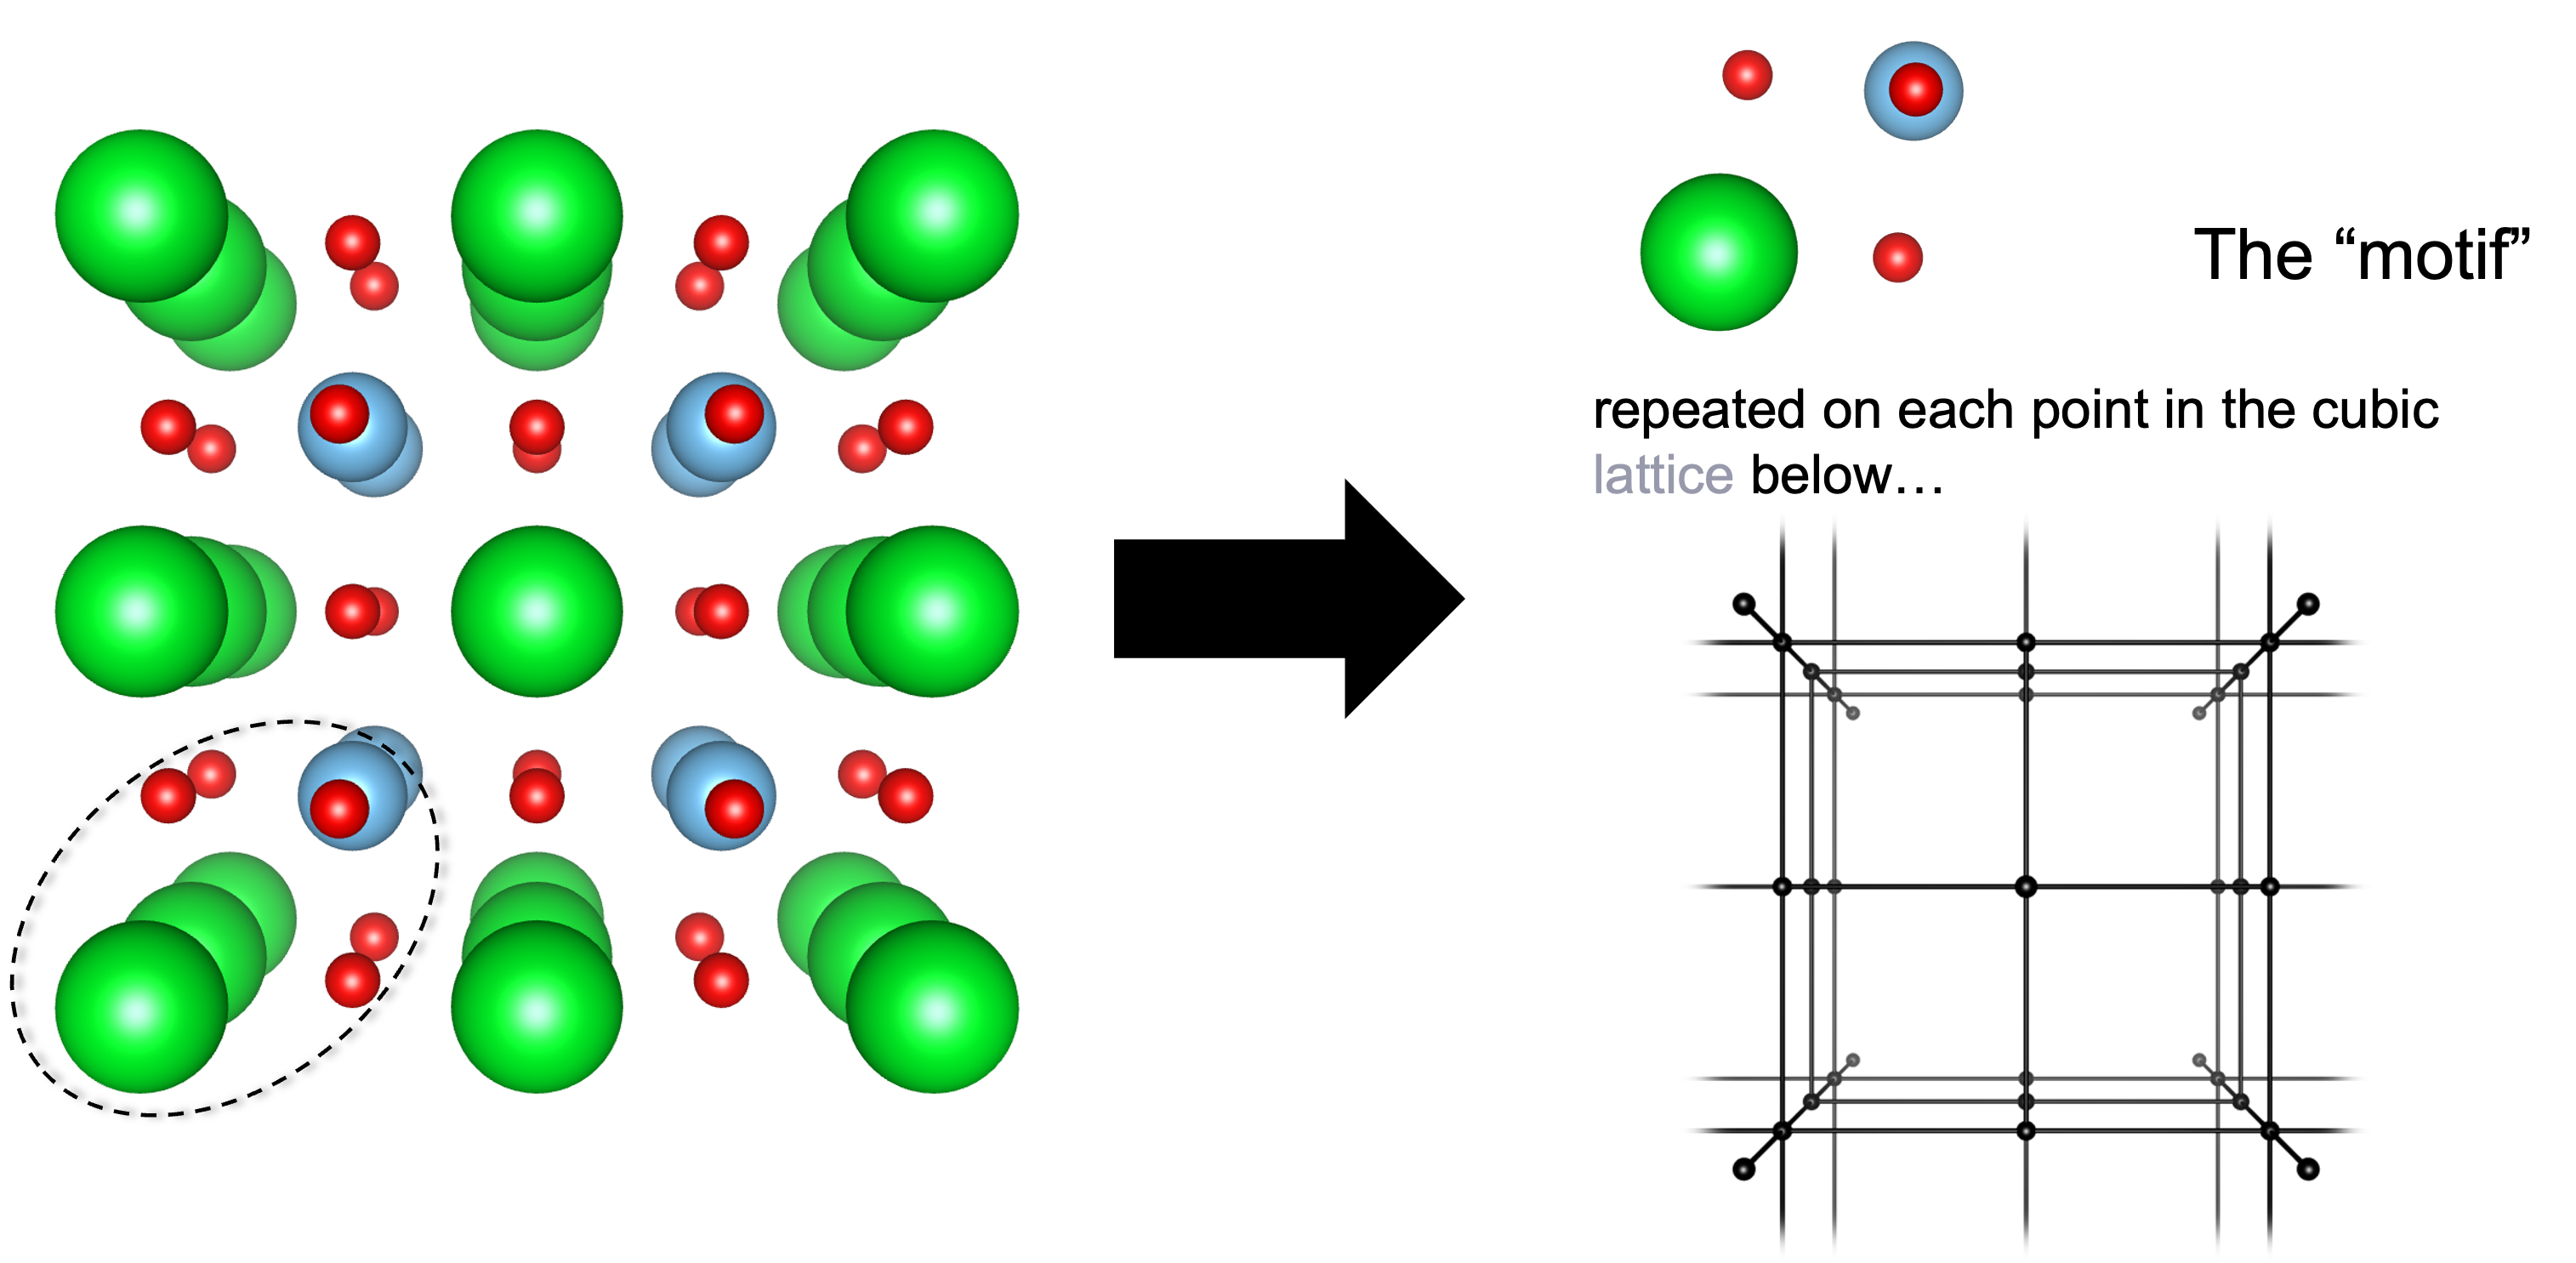
\includegraphics[width=0.6\linewidth]{lectures/figures/7_crystal.png}
    \caption{Perovskite \ce{SrTiO3}}
\end{figure}

\end{frame}


\begin{frame}{Translational symmetry}
All crystals are characterized by translational symmetry

\begin{equation*}
    \vec{t} = u \vec{a} + v \vec{b} + w \vec{c}, u, v, w \in \mathbb{Z}
\end{equation*}

\begin{figure}
    \centering
    \begin{subfigure}{0.25\textwidth}
        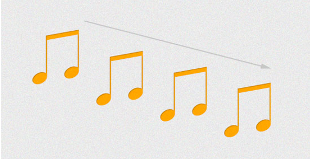
\includegraphics[width=\linewidth]{lectures/figures/7_1D_crystal.png}
    \caption{1D}
    \end{subfigure}
    \begin{subfigure}{0.4\textwidth}
        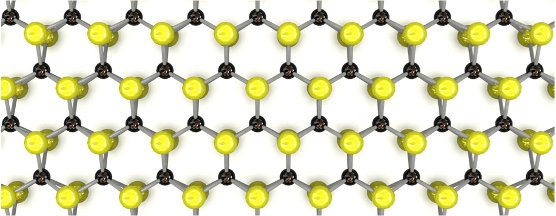
\includegraphics[width=\linewidth]{lectures/figures/7_2D_crystal.png}
    \caption{2D}
    \end{subfigure}
        \begin{subfigure}{0.25\textwidth}
        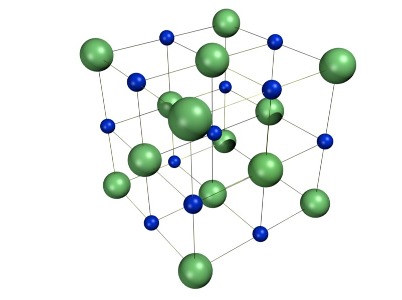
\includegraphics[width=\linewidth]{lectures/figures/7_3D_crystal.png}
    \caption{3D}
    \end{subfigure}
\end{figure}

\end{frame} 


\begin{frame}{The 14 3D Bravais Lattices}
\begin{columns}
\column{0.7\textwidth}
\begin{figure}
    \centering
    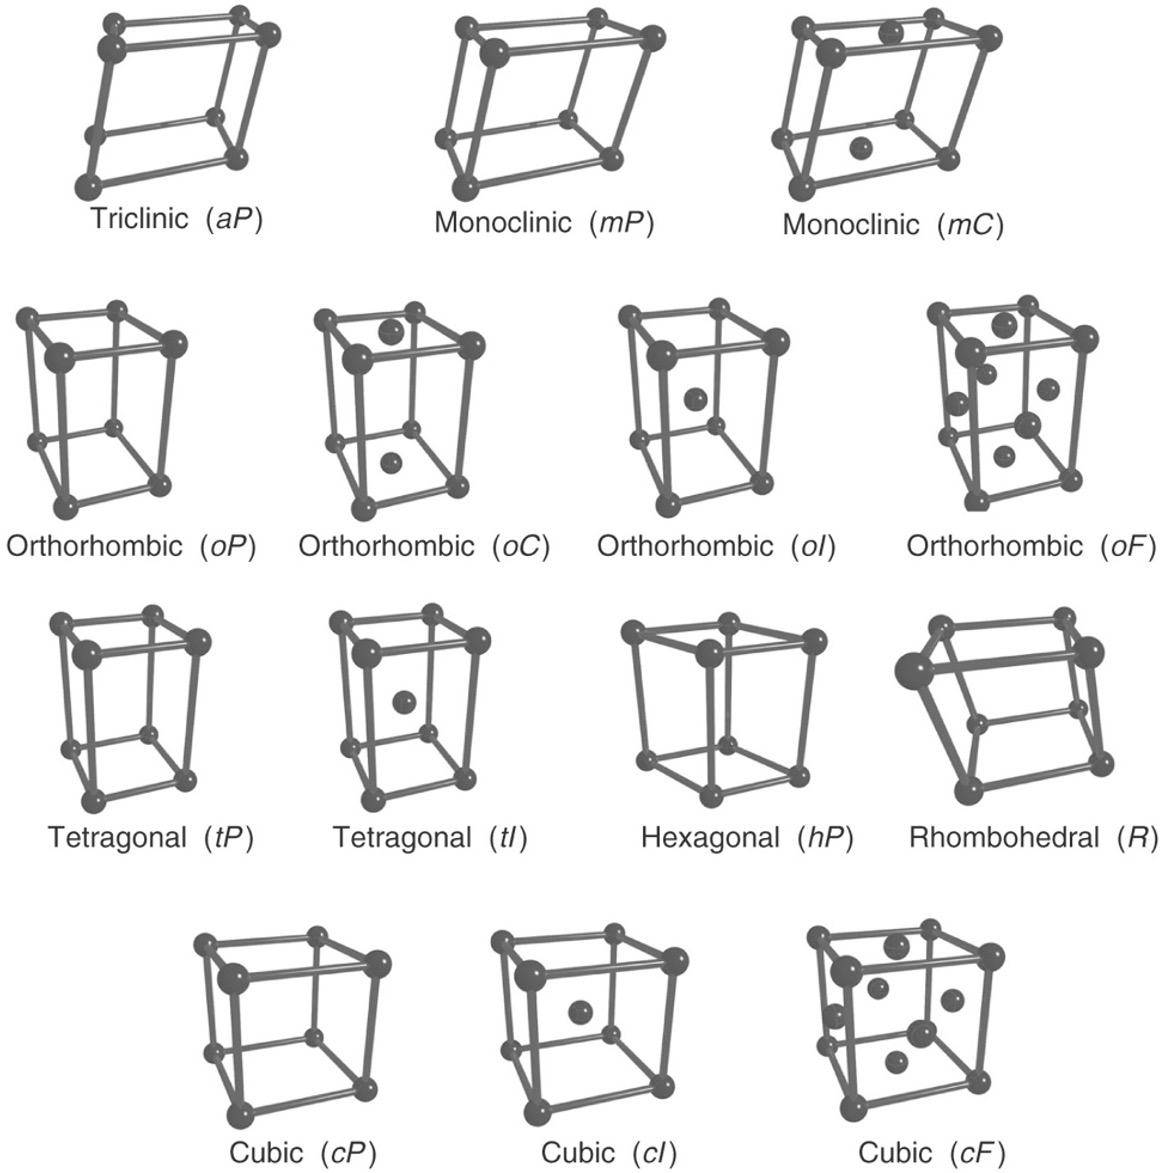
\includegraphics[width=0.6\linewidth]{lectures/figures/7_bravais_lattices.jpg}
\end{figure}
\column{0.3\textwidth}
a: triclinic (anorthic)\\
m: monoclinic\\
o: orthorhombic\\
t: tetragonal\\
h: hexagonal\\
c: cubic\newline
\newline
P: primitive\\
C: C-centered\\
I: body-centered\\
F: face-centered
\end{columns}

\end{frame} 

\begin{frame}{Unit cells}
Infinite number of unit cells for all 3D lattices. 

Always possible to define primitive unit cells for non-primitive lattices, though the full symmetry may not be retained.

\begin{figure}
    \centering
\begin{subfigure}{0.45\textwidth}
\centering
    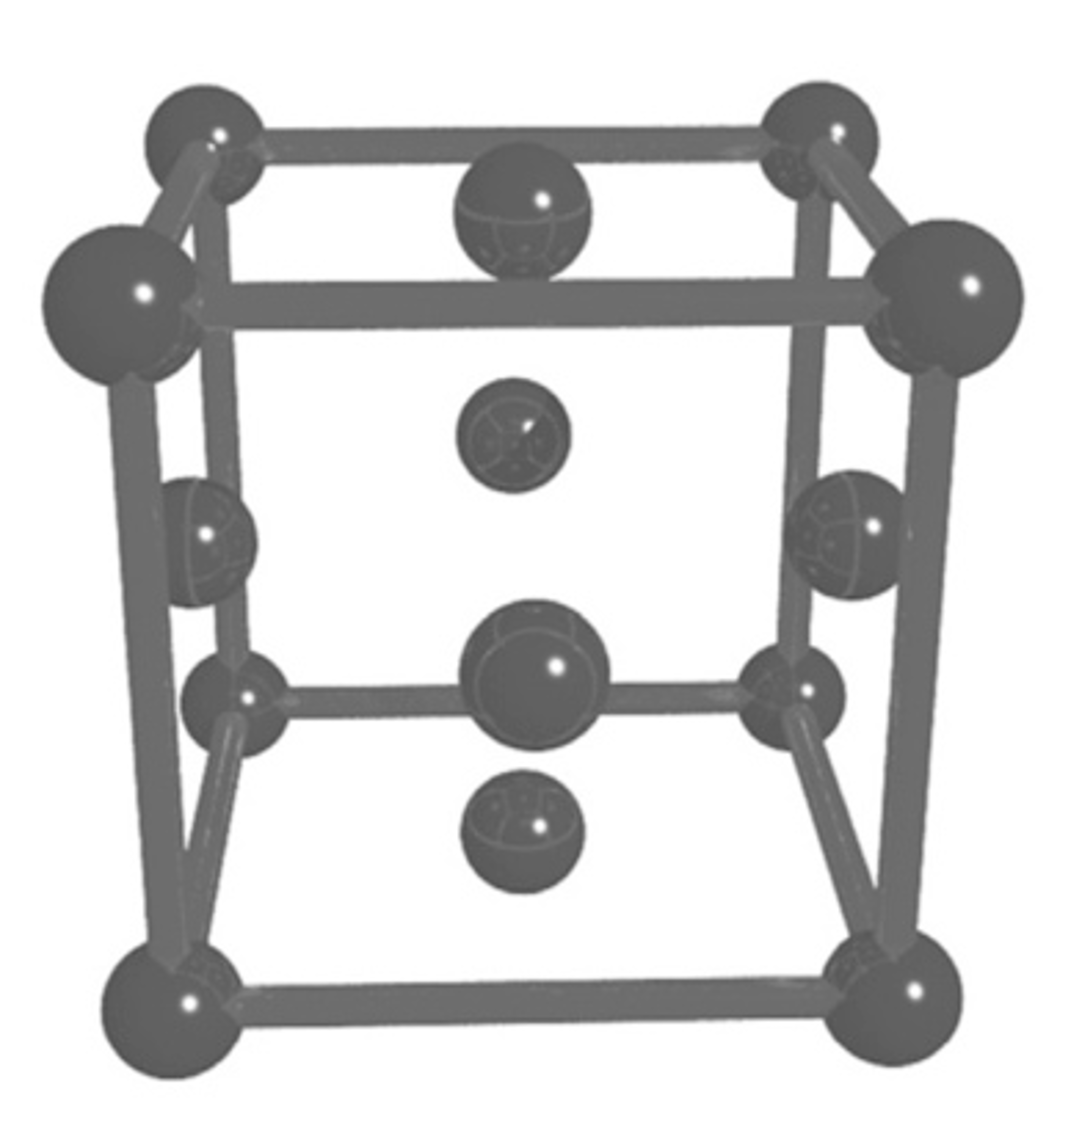
\includegraphics[width=0.6\textwidth]{lectures/figures/7_conventional_unit_cell.png}
    \caption{Conventional fcc cell}
\end{subfigure}
\begin{subfigure}{0.45\textwidth}
        \centering
        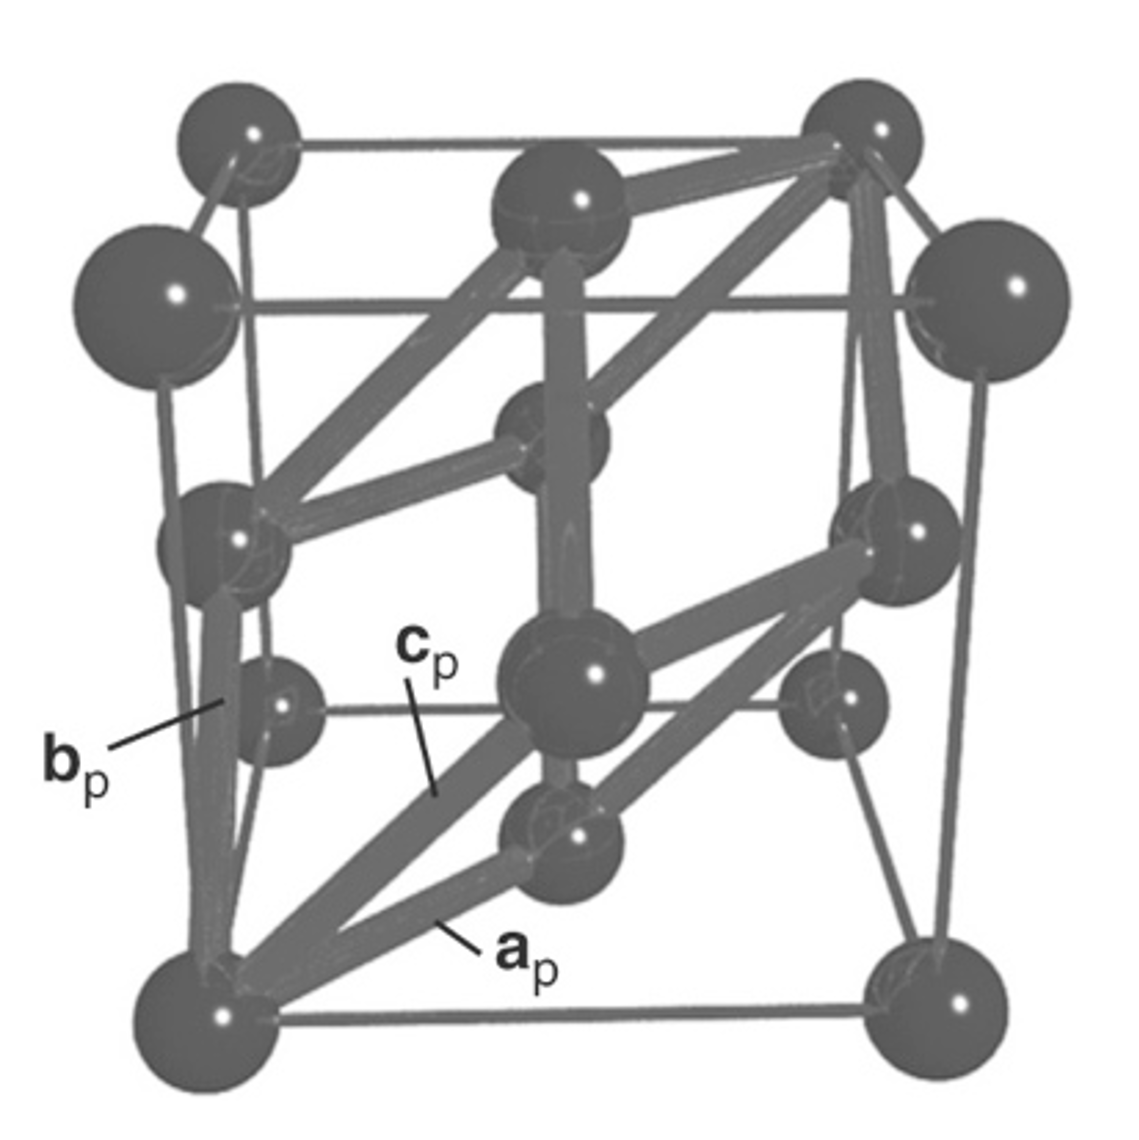
\includegraphics[width=0.6\textwidth]{lectures/figures/7_primitive_unit_cell.png}
    \caption{Primitive fcc cell}
\end{subfigure}
\end{figure}
\end{frame} 

\begin{frame}{Reciprocal Lattice}

\begin{columns}
\column{0.5\textwidth}
For a lattice given by basis vectors $\vec{a_1}$, $\vec{a_2}$ and $\vec{a_3}$, the reciprocal lattice is given basis vectors $\vec{a_1^*}$, $\vec{a_2^*}$ and $\vec{a_3^*}$ where:

\begin{eqnarray*}
    \vec{a_1^*} & = & 2\pi\frac{\vec{a_2} \times \vec{a_3}}{\vec{a_1}.(\vec{a_2} \times \vec{a_3})}\\
    \vec{a_2^*} & = & 2\pi\frac{\vec{a_3} \times \vec{a_1}}{\vec{a_1}.(\vec{a_2} \times \vec{a_3})}\\
    \vec{a_3^*} & = & 2\pi\frac{\vec{a_1} \times \vec{a_2}}{\vec{a_1}.(\vec{a_2} \times \vec{a_3})}
\end{eqnarray*}
\column{0.5\textwidth}
\begin{equation*}
    \vec{a_i^*}.\vec{a_j} = 2\pi \delta_{ij}
\end{equation*}

Reciprocal translation vectors are given by
\begin{equation*}
    \vec{G} = h\vec{a_1^*} + k\vec{a_2^*} + l\vec{a_3^*}
\end{equation*}
\end{columns} 

\end{frame}

\begin{frame}{External Potential for a Periodic Boundary System}

\begin{figure}
    \centering
    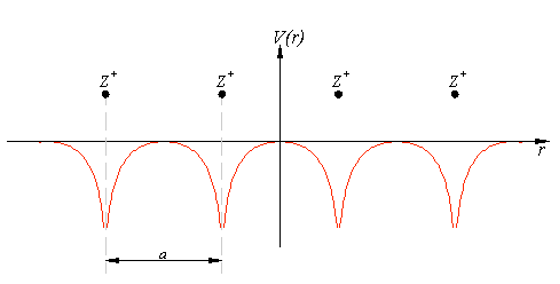
\includegraphics[width=0.8\linewidth]{lectures/figures/7_periodic_potential.png}
    \caption{Simple 1D periodic example}
\end{figure}

\end{frame}

\begin{frame}{Electron in a Periodic Potential}

For an electron in a 1D periodic potential with lattice vector $\vec{a}$, we have

\begin{equation*}
    H = - \frac{1}{2} \nabla^2 + V(r)
\end{equation*}

where $V(r)$ is periodic in $a$,

\begin{equation*}
    V(r) = V(r + ma), \forall m \in \mathbb{Z}
\end{equation*}

For any periodic function, we may express it in terms of a Fourier series:

\begin{equation*}
    V(r) = \sum_{n=-\infty}^{\infty} V_n e^{i\frac{2\pi}{a}nr}
\end{equation*}


\end{frame} 

\begin{frame}{Bloch's Theorem}
For a particle in a periodic potential, eigenstates can be written in the form of a Bloch wave:

\begin{equation*}
\psi_{n,\vec{k}}(\vec{r}) = e^{i\vec{k}.\vec{r}}u_{n,\vec{k}}(\vec{r})
\end{equation*} 

where $u_{n,\vec{k}}(\vec{r})$ has the same periodicity as the crystal and $\vec{k}$ is a vector of real numbers known as the \textbf{crystal wave vector}, $n$ is known as the \textbf{band index}. $e^{i\vec{k}.\vec{r}}$ is a ``plane wave''.\newline
\newline

For any reciprocal lattice vector $\vec{K}$, $\psi_{n,\vec{k}+\vec{K}}(\vec{r}) = \psi_{n,\vec{k}}(\vec{r})$, i.e., we only need to care about $\vec{k}$ in the first Brillouin Zone (BZ).

\end{frame} 


\begin{frame}{First BZ for Some Common Lattices}

\begin{figure}
    \centering
    \begin{subfigure}{0.24\textwidth}
        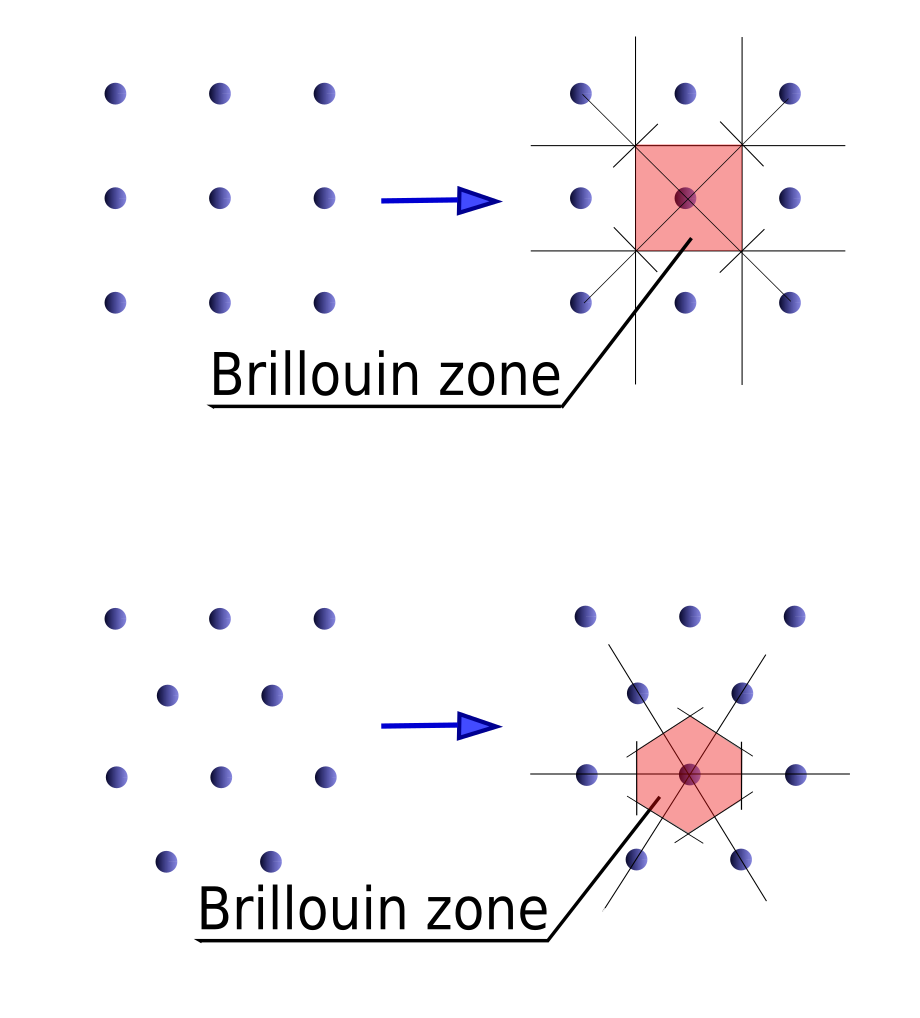
\includegraphics[width=\linewidth]{lectures/figures/7_Brillouin_Zone_2D.png}
    \caption{2D square and hex}
    \end{subfigure}
    \begin{subfigure}{0.24\textwidth}
        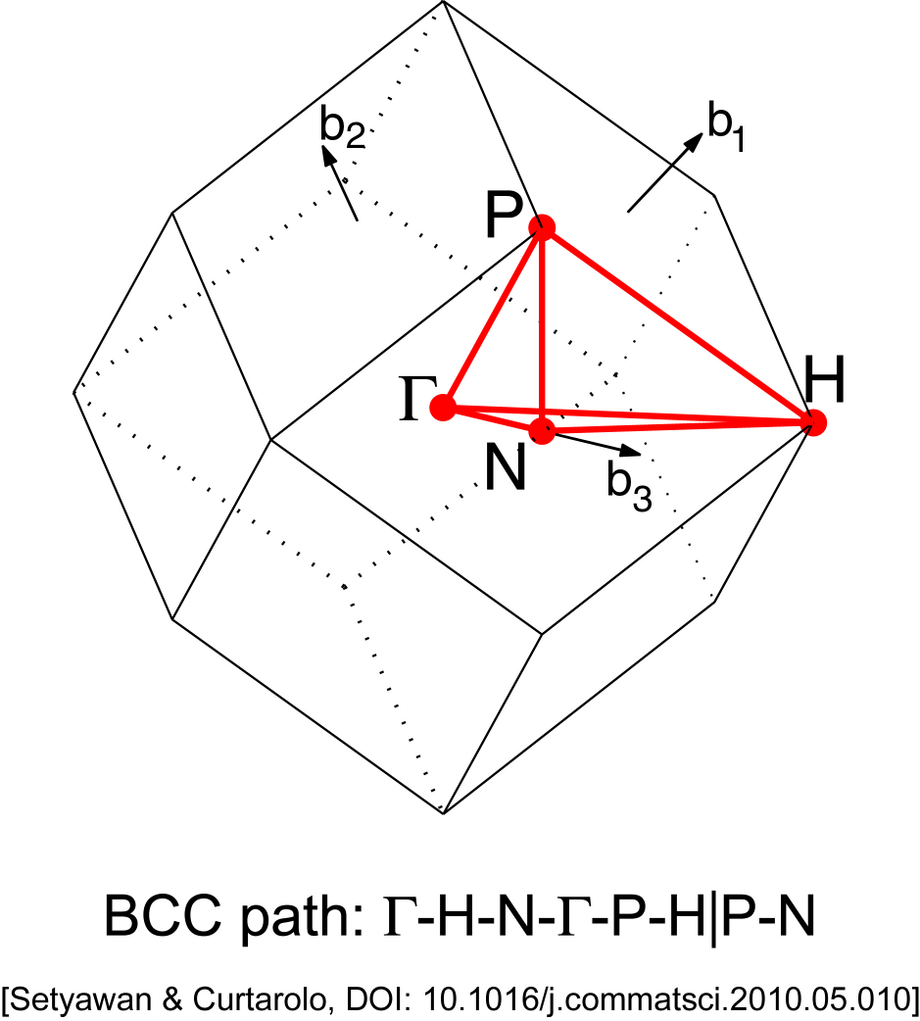
\includegraphics[width=\linewidth]{lectures/figures/7_Brillouin_Zone_BCC.png}
    \caption{BCC}
    \end{subfigure}
    \begin{subfigure}{0.24\textwidth}
        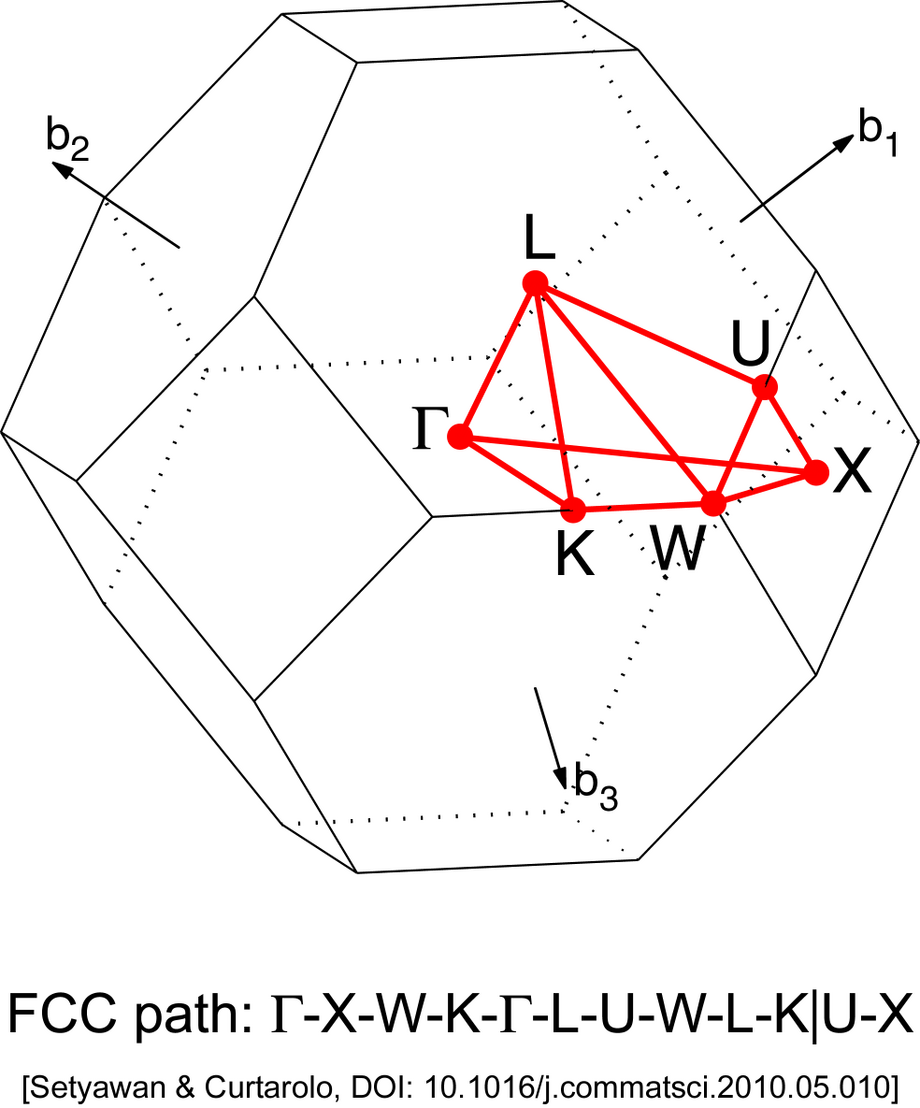
\includegraphics[width=\linewidth]{lectures/figures/7_Brillouin_Zone_FCC.png}
    \caption{FCC}
    \end{subfigure}
    \begin{subfigure}{0.24\textwidth}
        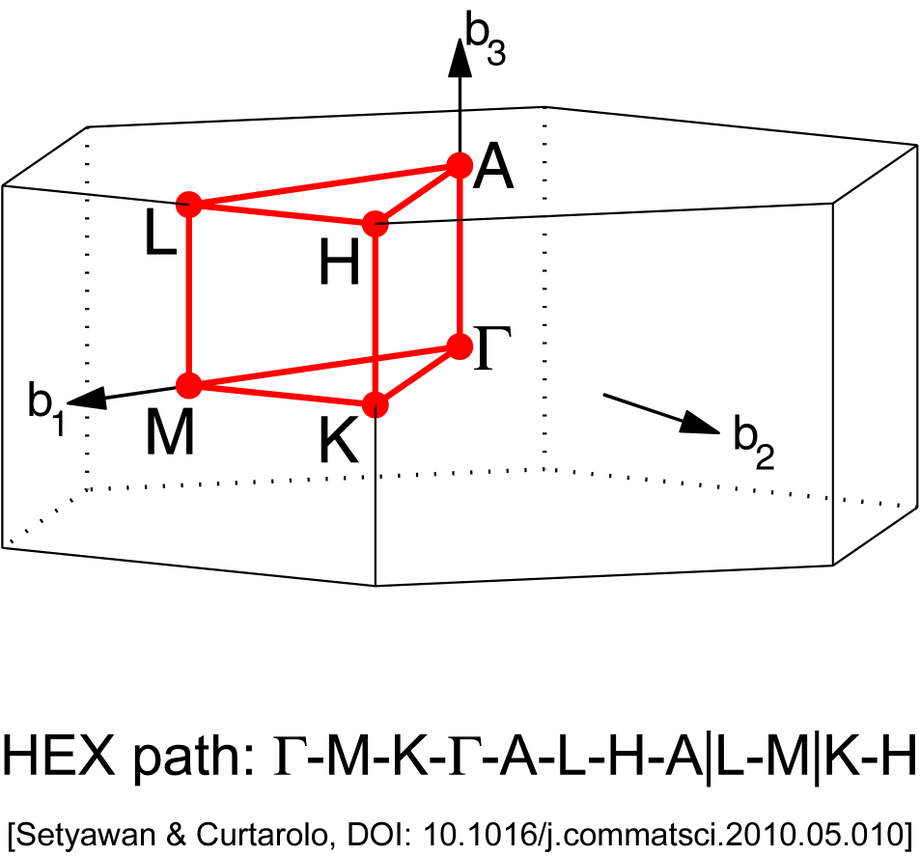
\includegraphics[width=\linewidth]{lectures/figures/7_Brillouin_Zone_Hex.png}
    \caption{Hexagonal}
    \end{subfigure}
\end{figure} 

\end{frame} 

\begin{frame}{Bloch Waves}
\begin{figure}
    \centering
    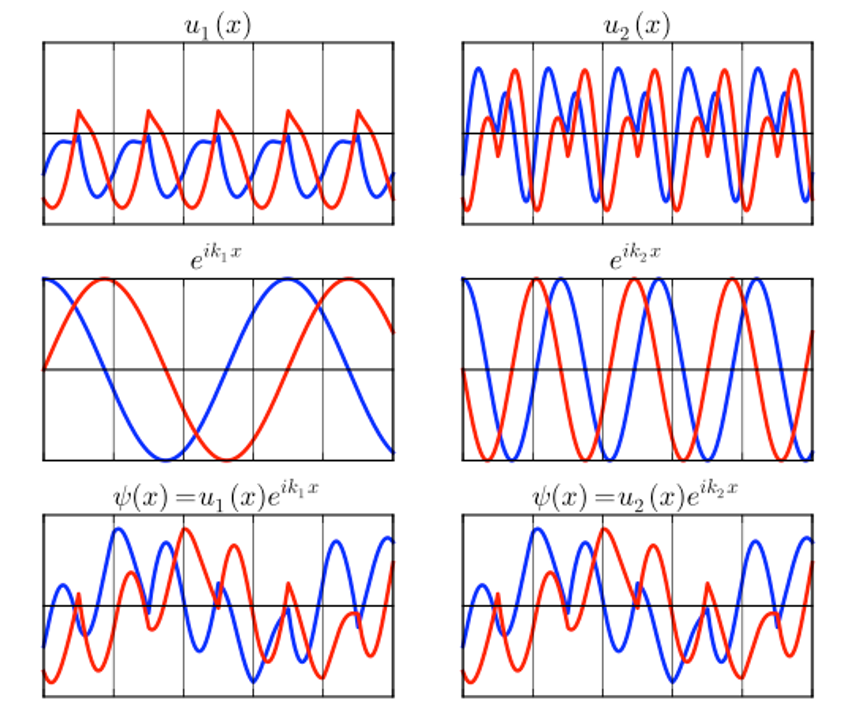
\includegraphics[width=0.5\linewidth]{lectures/figures/7_Bloch_Waves.png}
\end{figure} 
\end{frame} 

\begin{frame}{Plane Waves as a Basis}

From Bloch's Theorem, 
\begin{equation*}
\psi_{n,\vec{k}}(\vec{r}) = e^{i\vec{k}.\vec{r}}u_{n,\vec{k}}(\vec{r})
\end{equation*} 

Since $u_{n,\vec{k}}(\vec{r})$ has the same periodicity as the lattice, it can be written as a Fourier series of the reciprocal lattice:
\begin{eqnarray*}
u_{n,\vec{k}}(\vec{r}) & = & \sum_{\vec{G}} c^{\vec{G}}_{n,\vec{k}} e^{i\vec{G}.\vec{r}}
\end{eqnarray*} 

where $\vec{G} = h \vec{a_1^*} + k \vec{a_2^*} + l \vec{a_3^*}$ is a translation vector in the reciprocal lattice. Plugging this into the first equation, we have:

\begin{equation*}
\psi_{n,\vec{k}}(\vec{r}) = \sum_{\vec{G}} c^{\vec{G}}_{n,\vec{k}} e^{i(\vec{k}+\vec{G}).\vec{r}}
\end{equation*} 

Note that the summation is an infinite one over all reciprocal space translation vectors $\vec{G}$.

\end{frame} 

\begin{frame}{Truncating Plane Waves}

Plane waves offer a systematic way to improve completeness of our solution based on energy. \newline
\newline
For a free electron in a box, the solution to the Scr\"odinger equation is given by:

\begin{eqnarray*}
\psi(\vec{r}) = e^{i\vec{k}.\vec{r}}, E = \frac{\bar{h}^2}{2m}k^2
\end{eqnarray*} 

Analagously, the solution to to the Scr\"odinger equation for a periodic potential is a linear combination of plane waves with corresponding energies:
\begin{eqnarray*}
E_{\vec{k}+\vec{G}} = \frac{\bar{h}^2}{2m}|\vec{k}+\vec{G}|^2
\end{eqnarray*} 

\end{frame} 

\begin{frame}{Energy cutoff}
Solutions with lower energy are more physically important than solutions with higher energies. So we specify an energy cutoff:
\begin{eqnarray*}
E_{cut} = \frac{\bar{h}^2}{2m}|\vec{G}_{cut}|^2
\end{eqnarray*}

In PWSCF, this is specified using the \href{https://www.quantum-espresso.org/Doc/INPUT_PW.html}{``ecutwfc''} parameter. In the Vienna Ab Initio Simulation Package (VASP), it is called \href{https://www.vasp.at/wiki/index.php/ENCUT}{``ENCUT''}.\newline
\newline
Our wave function is then given by a \textit{finite} sum:

\begin{equation*}
\psi_{n,\vec{k}}(\vec{r}) = \sum_{|\vec{k}+\vec{G}<\vec{G_{cut}}|} c^{\vec{G}}_{n,\vec{k}} e^{i(\vec{k}+\vec{G}).\vec{r}}
\end{equation*} 

\end{frame} 

\begin{frame}{Convergence with respect to energy cutoff}
\begin{columns}
\column{0.5\textwidth}
\begin{figure}
    \centering
    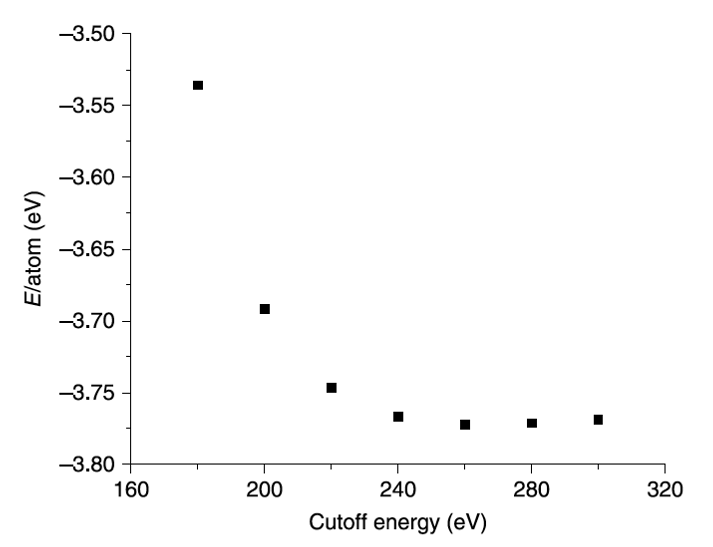
\includegraphics[width=0.8\linewidth]{lectures/figures/7_convergence_energy_cutoff.png}
    \caption{Energy per atom of fcc Cu with lattice constant of 3.64 \AA~using a $12 \times 12 \times 12$ $k$ points as a function of energy cutoff.\cite{shollDensityFunctionalTheory2009}}
\end{figure} 
\column{0.5\textwidth}
\begin{alertblock}{Basis Set Consistency}
The same energy cutoff should be used to ensure basis set consistency if you want to compare energies between calculations, e.g.:

\ce{Cu (s) + Pd (s) -> CuPd(s)}
\end{alertblock}
\end{columns} 

\end{frame} 


\begin{frame}{Pseudopotentials (PSPs)}
\begin{columns}

\column{0.4\textwidth}

\begin{figure}
    \centering
    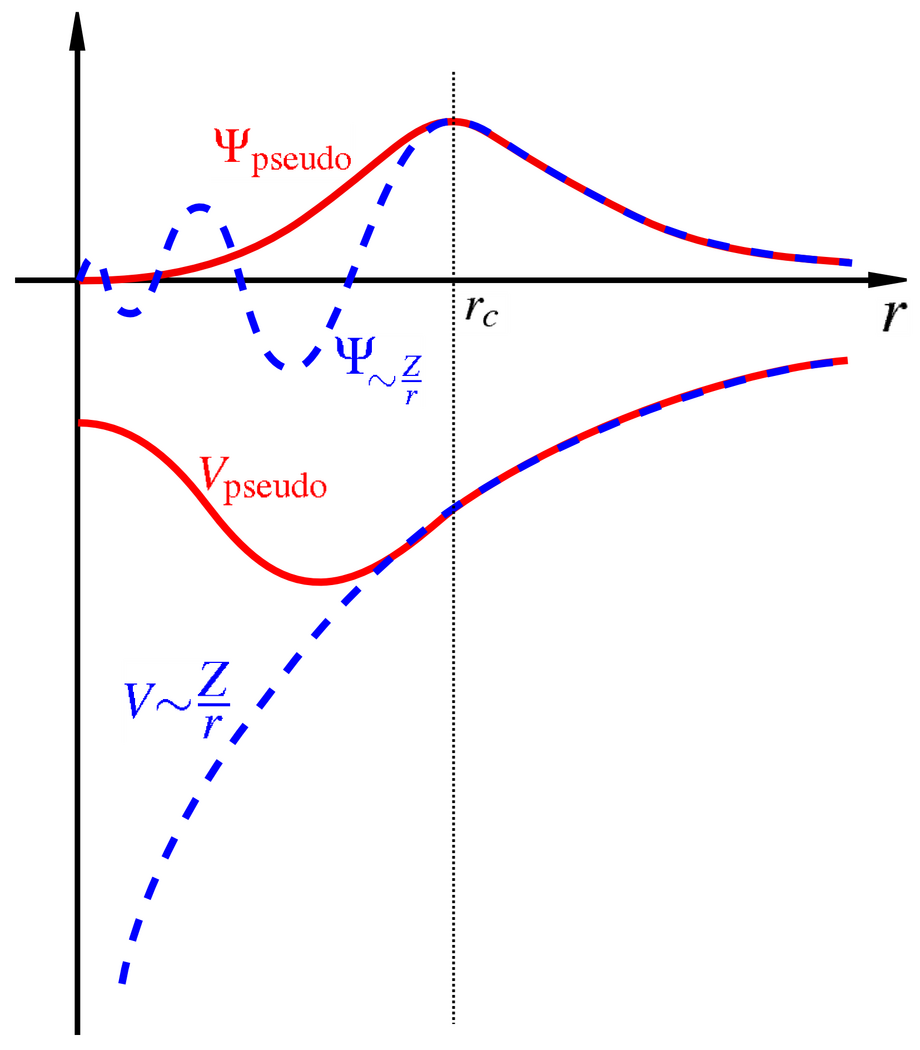
\includegraphics[width=0.6\linewidth]{lectures/figures/7_Pseudopotentials.png}
    \caption{Comparison of the real (blue) and pseudo (red) wavefunctions. The potentials match above the cutoff radius.}
\end{figure} 

\column{0.6\textwidth}
\begin{equation*}
\psi_{n,\vec{k}}(\vec{r}) = \sum_{\vec{G}} c^{\vec{G}}_{n,\vec{k}} e^{i(\vec{k}+\vec{G}).\vec{r}}
\end{equation*} 
\textbf{Problem: }Tightly bound electrons have wavefunctions that oscillate on very short length scales $\implies$ Need a huge cutoff (and lots of plane waves).\newline
\newline
\textbf{Solution:} Pseudopotentials (PSPs) to represent core electrons with a smoothed density to match various important physical and mathematical properties of true ion core.

\end{columns} 
\end{frame} 

\begin{frame}{Types of Pseudopotentials}

\begin{columns}
\column{0.4\textwidth}
\textbf{Norm-conserving (NC)}: Enforces that inside cut-off radius, the norm of the pseudo-wavefunction is identical to the all-electron wavefunction.\newline
\newline
\textbf{Ultrasoft (US)}: Relax NC condition to reduce basis set size further.\newline
\newline
\textbf{Projector-augmented wave (PAW)}: Avoid some problems with USPP
Generally gives similar results as USPP and all-electron in many instances.\cite{kresseUltrasoftPseudopotentialsProjector1999}
\column{0.6\textwidth}
\begin{figure}
    \centering
        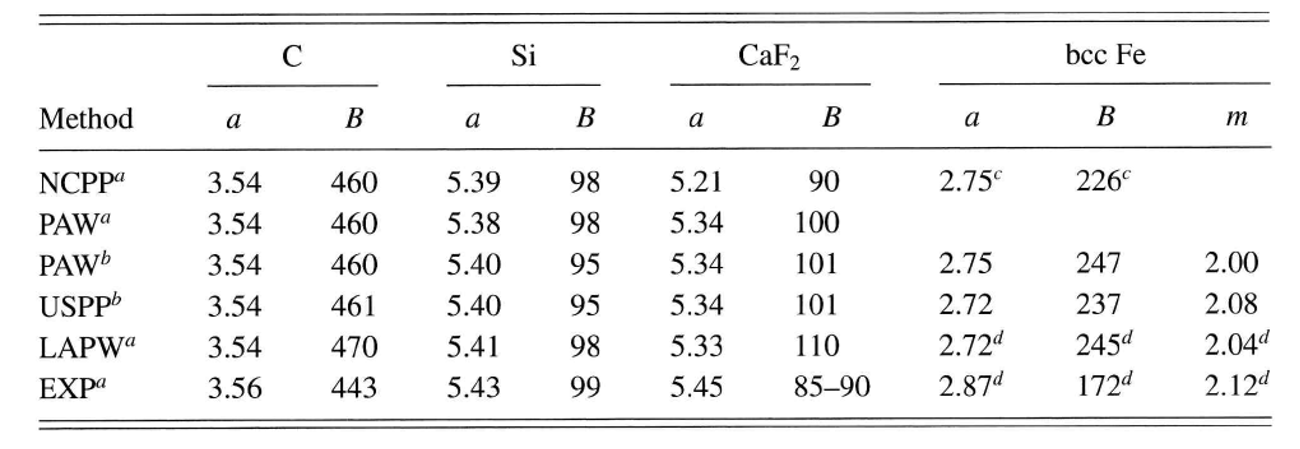
\includegraphics[width=\linewidth]{lectures/figures/7_PSP_comparison.png}
    \caption{Calculated properties of selected crystals using LDA: norm-conserving pseudopotentials (NCPPs), projector augmented waves (PAWs), ultrasoft pseudopotentials (USPPs) and linearized APWs.}
\end{figure} 

\end{columns} 

\end{frame} 

\begin{frame}{Choosing PSPs}
Sometimes, several PPs are available with different number of ``valence'' electrons, i.e., electrons not in the core.\newline
\newline
Choice depends on research problem – if you are studying problems where more (semi-core) electrons are required, choose PSP with more electrons.\newline
\newline
But more electrons $\neq$ better results! (e.g., Rare-earth elements)

\end{frame} 


\begin{frame}{Integrations in $k$ space}
For counting of electrons in bands, total energies, etc., need to sum/intergate over states labeled by $\vec{k}$:
\begin{equation*}
<f> = \frac{V_{cell}}{2\pi} \int_{BZ} f(\vec{k}) d\vec{k} \approx \frac{V_{cell}}{2\pi} \sum_{\vec{k}} f(\vec{k})
\end{equation*} 

\textbf{Born-von Karman boundary condition}: For large but finite crystal of volume $V$ with edges $N_1 \vec{a_1}$, $N_2 \vec{a_2}$, $N_1 \vec{a_3}$:

\begin{equation*}
\psi(\vec{r} + N_1 \vec{a_1}) = \psi(\vec{r} + N_2 \vec{a_2}) = \psi(\vec{r} + N_3 \vec{a_3}) = \psi(\vec{r})
\end{equation*} 

For our Bloch plane waves, the compatible set of $\vec{k}$ is given by:
\begin{equation*}
e^{i\vec{k}.(\vec{r} + N_i \vec{a_i})} = e^{i\vec{k}.\vec{r}}\implies e^{i\vec{k}.N_i \vec{a_i}} = 1 \implies \vec{k} = \frac{m_1}{N_1} \vec{g_1} +  \frac{m_2}{N_2} \vec{g_2} +\frac{m_3}{N_3} \vec{g_3}
\end{equation*} 

\end{frame} 


\begin{frame}{Choosing $\vec{k}$ point grids}

\textbf{Sampling at one point}
\begin{itemize}
    \item Baldereschi point: Point such that the value which any given periodic function of wave vector assumes at this point is an excellent approximation to the average value of the same function throughout the Brillouin zone. This special point is termed the ``mean-value point'' and is dictated by the crystal symmetry. The coordinates of the mean-value point for cubic lattices are explicitly given.
    \item Gamma ($\Gamma$) point: 
\end{itemize}

\textbf{Sampling in a Grid}
\begin{itemize}
    \item Monkhorst-Pack – Sampling at regular grid mesh.
    \item Special grids along 
\end{itemize}

\end{frame} 



    \begin{frame}[allowframebreaks]{Bibliography}
        \bibliographystyle{unsrt}
        \bibliography{refs}
    \end{frame}



    \begin{frame}
        \Huge{\centerline{The End}}
    \end{frame}

\end{document}

